%\documentclass[manuscript]{acmart}
%\documentclass[acmsmall]{acmart}
%\settopmatter{printacmref=false}


\documentclass[
  a4paper,
  12pt,
  DIV=12,        % höherer Wert = schmalere Ränder, weniger Whitespacmi
  parskip=half,  % Absätze mit halbem Abstand statt Einzug
  headings=small % kleinere Überschriften, weniger vertikaler Abstand
]{scrartcl}

%\documentclass[a4paper,11pt]{scrartcl}
%\documentclass[a4paper,11pt]{report}
%\documentclass[a4paper,12pt]{book}
\usepackage[utf8]{inputenc}
\usepackage[german]{babel}
\usepackage[T1]{fontenc}
\usepackage{lmodern}
\usepackage{graphicx}
\usepackage{amsmath}
\usepackage{caption}
\usepackage{gensymb}
\usepackage{microtype}
\usepackage{longtable}
\usepackage{tabularx}   % Spalten, die die restliche Zeilenbreite auffüllen (X-Spalte)
\usepackage{booktabs}   % \toprule \midrule \bottomrule (in mobrob_table.tex verwendet)
\usepackage{wrapfig}    % Textumfluss um Abbildungen
\usepackage{array}
\usepackage{calc}

\usepackage[citecolor=black, colorlinks=true, linkcolor=black, urlcolor=blue]{hyperref}


%\usepackage{geometry}
\usepackage{siunitx}
%\geometry{margin=2.5cm}


\usepackage{amsthm}
\usepackage{mdframed}
\usepackage{enumitem}

\newmdtheoremenv{theorem}{Theorem}

\theoremstyle{definition}
\newmdtheoremenv{derivation}{Derivation}

\providecommand{\tightlist}{%
  \setlength{\itemsep}{0pt}\setlength{\parskip}{0pt}}

%\mdfdefinestyle{leftline}{
%    topline=false, bottomline=false, rightline=false,
%    linewidth=2pt, linecolor=gray
%}
\theoremstyle{definition}
\newmdtheoremenv[style=leftline]{myalgorithm}{Algorithm}




%\usepackage{fancyvrb}







\let\Bbbk\relax
\usepackage{amssymb}


\usepackage{yfonts}

\usepackage{kvmap}

\usepackage[
    backend=biber,
    style=alphabetic,
    sortlocale=de_DE,
    natbib=true,
    %url=false,
    doi=true,
    %eprint=false
]{biblatex}
\addbibresource{literatur.bib}

%\usepackage[
%    backend=biber,
%    style=alphabetic,
%    sortlocale=de_DE,
%    natbib=true,
%    %url=false,
%    doi=true,
%    %eprint=false
%]{biblatex}
%\addbibresource{Literaturrecherche-Dennis/mobrob_references.bib}

\usepackage[autostyle=true,german=quotes]{csquotes}
\usepackage{trfsigns} %fourier transform arrow
\usepackage{mathrsfs} %fourier F
\usepackage{commath}

\usepackage{pgfplots}
\pgfplotsset{compat=1.18}

\usepackage{xcolor}
\usepackage{listings}
\usepackage[european]{circuitikz}
\ctikzset{tripoles/european not symbol=ieee circle}

%\usepackage[shading]{moeptikz}
%\moeptikzset{shading=true}

%\usepackage{german,longtable}

\usepackage{xcolor}
\usepackage{color}
\usepackage{url}

\usepackage{xfrac}

\usepackage{listings}
\usepackage{verbatimbox}

\usepackage{algorithm}
\usepackage{algpseudocode}

\usepackage{multirow}
\usepackage{float}
\usepackage{pdflscape}   % einzelne Querformatseiten (im PDF gedreht)

%%%% TIKZ

\usepackage{tikz}

\usepackage{pgfplots}
\usetikzlibrary{calc,
trees,positioning,arrows,
chains,shapes.geometric,
decorations.pathreplacing,
decorations.pathmorphing,shapes,
matrix,shapes.symbols,
plotmarks}
%\tikzexternalize[prefix=figures/]

%\tikzset{%
%  block/.style    = {draw, thick, rectangle, minimum height = 3em,
%    minimum width = 3em},
%  sum/.style      = {draw, circle, node distance = 2cm}, % Adder
%  input/.style    = {coordinate}, % Input
%  output/.style   = {coordinate} % Output
%}
% Defining string as labels of certain blocks.
%\newcommand{\suma}{\Large$+$}
%\newcommand{\multa}{\Large$\times$}
%\newcommand{\inte}{$\displaystyle \int$}
%\newcommand{\derv}{\huge$\frac{d}{dt}$}

\usetikzlibrary{arrows,automata,positioning}
%\usepackage{automata}


%%% END TIKZ

\usepackage[section]{placeins}

\usepackage{textcomp}


\usepackage{listings}
\usepackage{verbatimbox}

\usepackage{bold-extra}

\usepackage{framed}

%\usepackage{fancyhdr}
%\pagestyle{fancy}
%\lhead{\leftmark}
%\chead{}
%\rhead{}
%\lfoot{}
%\cfoot{\thepage}
%\rfoot{}
%\renewcommand{\headrulewidth}{0.2pt}
%\renewcommand{\footrulewidth}{0.2pt}



\newcommand{\Z}{\mathbb{Z}}
\newcommand{\R}{\mathbb{R}}
\newcommand{\C}{\mathbb{C}}
\newcommand{\N}{\mathbb{N}}
\newcommand{\SqrtNy}{$\sqrt{\textsc{Ny}}$}
\newcommand{\conj}{\overline}
\newcommand{\Kset}{\textswab{K}}
\newcommand{\Qset}{\textswab{Q}}
\newcommand{\ceil}[1]{\left\lceil #1 \right\rceil}
\newcommand{\floor}[1]{\left\lfloor #1 \right\rfloor}
\newcommand{\sorted}[1]{\textsc{sort}\left\lbrace #1 \right\rbrace}
\newcommand{\SNRgain}{a_{SNR}}
\newcommand{\EQgain}{a_{EQ}}
\newcommand{\SIRgain}{a_{SIR}}
\newcommand{\SNIRgain}{a_{SINR}}
\newcommand{\SNR}{\textsc{SNR}}
\newcommand{\CIRgain}{a_{CIR}}
\newcommand{\CINRgain}{a_{CINR}}
\newcommand{\CNR}{\textsc{CNR}}
\newcommand{\CINR}{\textsc{CINR}}
\newcommand{\HPAModel}{ Hughes 1177H TWTA }
\newcommand{\bigO}{\mathcal{O}}
\newcommand{\CopWinCompl}{2.375377}
\newcommand{\IBO}{\textsc{IBO}}
\newcommand{\OBO}{\textsc{OBO}}
\newcommand{\spacepage}{\newpage\null\thispagestyle{empty}\newpage}
\newcommand{\satcom}{ SatCom }
\newcommand{\db}{~\text{dB}}


\definecolor{mGreen}{rgb}{0,0.6,0}
\definecolor{mGray}{rgb}{0.5,0.5,0.5}
\definecolor{mPurple}{rgb}{0.58,0,0.82}
\definecolor{backgroundColour}{rgb}{0.95,0.95,0.92}

\lstdefinestyle{CStyle}{
    backgroundcolor=\color{backgroundColour},
    commentstyle=\color{mGreen},
    keywordstyle=\color{magenta},
    numberstyle=\tiny\color{mGray},
    stringstyle=\color{mPurple},
    basicstyle=\footnotesize,
    breakatwhitespace=false,
    breaklines=true,
    captionpos=b,
    keepspaces=true,
    numbers=left,
    numbersep=5pt,
    showspaces=false,
    showstringspaces=false,
    showtabs=false,
    tabsize=2,
    language=C
}

\lstdefinelanguage{VHDL}{
  morekeywords=[1]{library,use,all,entity,is,port,in,out,end,architecture,of,begin,process,if,then,else,elsif,when,others,signal,variable,wait,for,loop},
  morecomment=[l]--,
  morestring=[b]",
  sensitive=true
}

\lstset{
  language=VHDL,
  basicstyle=\ttfamily\small,
  keywordstyle=\color{blue},
  commentstyle=\color{gray},
  stringstyle=\color{red},
  numbers=left,
  numberstyle=\tiny,
  stepnumber=1,
  numbersep=8pt,
  frame=single,
  breaklines=true,
  captionpos=b
}

\lstset{numbers=none}

%\newcounter{example}
%\renewcommand{\theexample}{\thesection.\arabic{example}}


% Default fixed font does not support bold face
\DeclareFixedFont{\ttb}{T1}{txtt}{bx}{n}{12} % for bold
\DeclareFixedFont{\ttm}{T1}{txtt}{m}{n}{12}  % for normal

% Custom colors
\usepackage{color}
\definecolor{deepblue}{rgb}{0,0,0.5}
\definecolor{deepred}{rgb}{0.6,0,0}
\definecolor{deepgreen}{rgb}{0,0.5,0}

\usepackage{listings}

% Python style for highlighting
\newcommand\pythonstyle{\lstset{
language=Python,
basicstyle=\ttm,
morekeywords={self},              % Add keywords here
keywordstyle=\ttb\color{deepblue},
emph={MyClass,__init__},          % Custom highlighting
emphstyle=\ttb\color{deepred},    % Custom highlighting style
stringstyle=\color{deepgreen},
frame=tb,                         % Any extra options here
showstringspaces=false
}}


% Python environment
\lstnewenvironment{python}[1][]
{
\pythonstyle
\lstset{#1}
}
{}

% Python for external files
\newcommand\pythonexternal[2][]{{
\pythonstyle
\lstinputlisting[#1]{#2}}}

% Python for inline
\newcommand\pythoninline[1]{{\pythonstyle\lstinline!#1!}}





\nocite{*}

\begin{document}

%\pagenumbering{roman}



\title{Coasterbot}
\subtitle{Konzeptbeschreibung}
\author{Dennis Borutta}
%\email{gereonsuch@suchdsp.com}
%\affiliation{
%  \institution{Wilhelm Büchner University of Applied Sciences}
%  \department{Computer Engineering}
%  \city{Hof}
%  \country{Germany}
%}



\begin{titlepage}
  \begin{center}
    {\large Wilhelm Büchner University of Applied Sciences} \\[0.3em]

    {\normalsize Projektseminar Master}
\vspace{5em}

    {\LARGE\bfseries Coasterbot} \\[0.5em]

    {\large Konzeptbeschreibung} \\[1em]

    {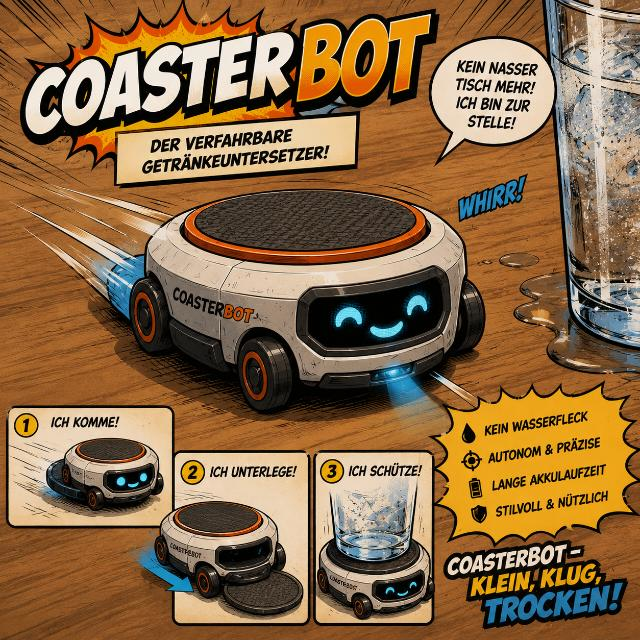
\includegraphics[width=0.38\textwidth]{coasterbot.png}} \\[1em]

\vspace{4em}

    {\normalsize
\begin{tabular}{ll}
Dennis Borutta, B. Eng & dennis.borutta@outlook.com\\
Stefan Etringer, B. Eng & mail@stefan.works\\
Gereon Such, M. Sc. & gereonsuch@gmail.com\\
\end{tabular}
    }
  \end{center}


\end{titlepage}


% einleitung preambel etc.


% Versionshistorie des Dokuments -- eigene Seite direkt nach dem Titelblatt
\section*{Versionshistorie}

\begin{tabularx}{\textwidth}{@{}clp{2.6cm}X@{}}
\toprule
\textbf{Version} & \textbf{Datum} & \textbf{Bearbeiter} & \textbf{Änderungen}\\
\midrule
1 & 24.08.2026 & Borutta & Erstfassung der Konzeptbeschreibung\\
\bottomrule
\end{tabularx}


\newpage

\tableofcontents

\newpage

\section{Konzeptbeschreibung}\label{coasterbot-konzeptbeschreibung}

\subsection{Übersicht}\label{uebersicht}

Der Coasterbot ist ein mobiler Roboter auf einem vierrädrigen Chassis,
dessen zentrale Funktion die \textbf{Aufnahme und Ausgabe von
Untersetzern} ist. Der Roboter ist mit einem Lochraster-Chassis
aufgebaut, das eine flexible Montage von Elektronik, Sensorik und
Mechanik erlaubt. Aus diesem Grund sind in den folgenden Bildern noch
nicht alle Komponenten sichtbar. Deren ideale Platzierung kann am
Prototyp variieren und so der optimale Platz gefunden werden. Vier
einzeln angetriebene Räder sorgen für die Fortbewegung, während im
Zentrum des Fahrzeugs ein Mechanismus zur Untersetzerhandhabung
untergebracht ist.

\subsection{Gesamtkonzept}\label{gesamtkonzept}

Die folgenden Ansichten zeigen das grundlegende Layout des Roboters
aus der Vogelperspektive sowie von vorne.

\subsubsection{Draufsicht (Konzept)}\label{draufsicht-konzept}

\begin{figure}
\centering
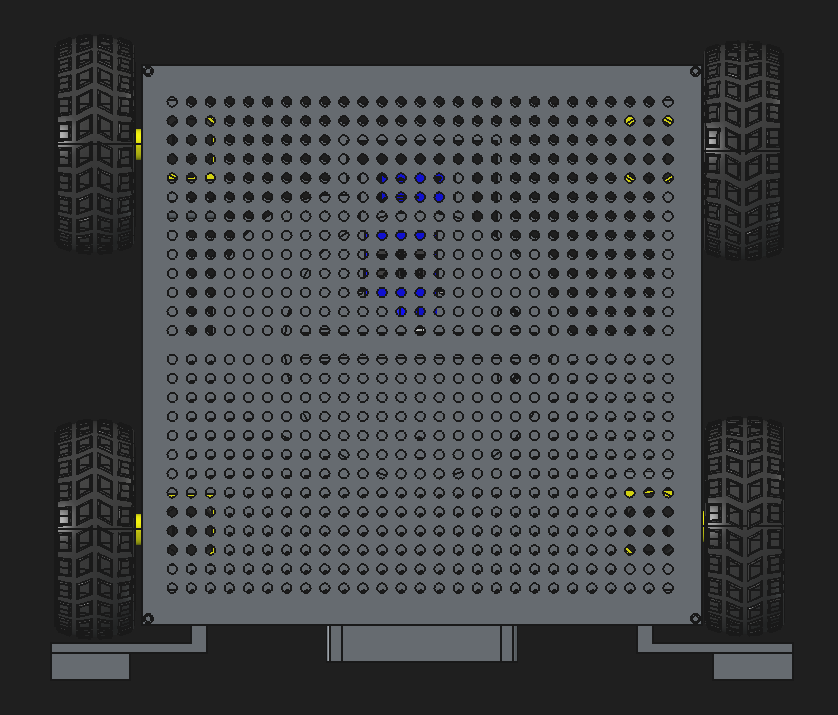
\includegraphics[width=0.75\textwidth,keepaspectratio,alt={Konzept Draufsicht}]{Konzept_Draufsicht.png}
\caption{Konzept Draufsicht}
\label{draufsicht-konzept}
\end{figure}

Die Draufsicht in Abbildung~\ref{draufsicht-konzept} zeigt die symmetrische Anordnung der vier Räder in den
Ecken des Chassis. Die blau durchscheinende Bereiche kennzeichnen die
Position der Servomotoren für die Ausgabe und Aufnahme von Untersetzer,
die gelb durchscheinenden Bereiche sind die verwendeten Antriebsmotoren
zur Fortbewegung. Befestigt wird die obere Platte über vier Schrauben an
das Grundgestell. Damit Klemmt diese obere Platte vier Seitenwände in
das Grundgestell ein.

\subsubsection{Frontansicht (Konzept)}\label{frontansicht-konzept}

\begin{figure}
\centering
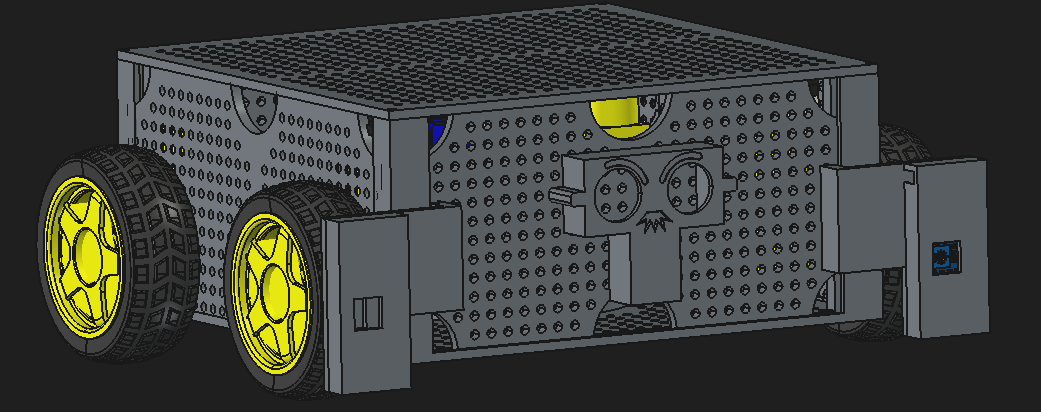
\includegraphics[width=0.75\textwidth,keepaspectratio,alt={Konzept schräge Frontansicht}]{Konzept_Frontansicht.png}
\caption{Konzept schräge Frontansicht}
\label{frontansicht-konzept}
\end{figure}

Die Frontansicht in Abbildung~\ref{frontansicht-konzept} verdeutlicht das Fahrzeug sowie die Anbringung der
Sensoren zur Kanten- und Hinderniserkennung. Mittig ist eine stilisierte
„Gesichts''-Blende zu erkennen, welche einen Ultraschallsensor aufnehmen
kann zur Hinderniserkennung. Die vor den Rädern stehenden Gehäuse sind
zur Aufnahme der Sensorik zur Kantenerkennung gedacht. Diese werden auch
für die hinteren Räder vorgesehen. Die Antriebsräder werden direkt mit
den Außenwänden verschraubt. Alle Außenwände werden von oben in das
Grundgestell eingeschoben. Die ist an den Führungen in den Eckpfeilern
erkennbar.

\subsection{Mechanischer Aufbau}\label{mechanischer-aufbau}

\subsubsection{Isometrische Ansicht ohne
Deckel}

\begin{figure}
\centering
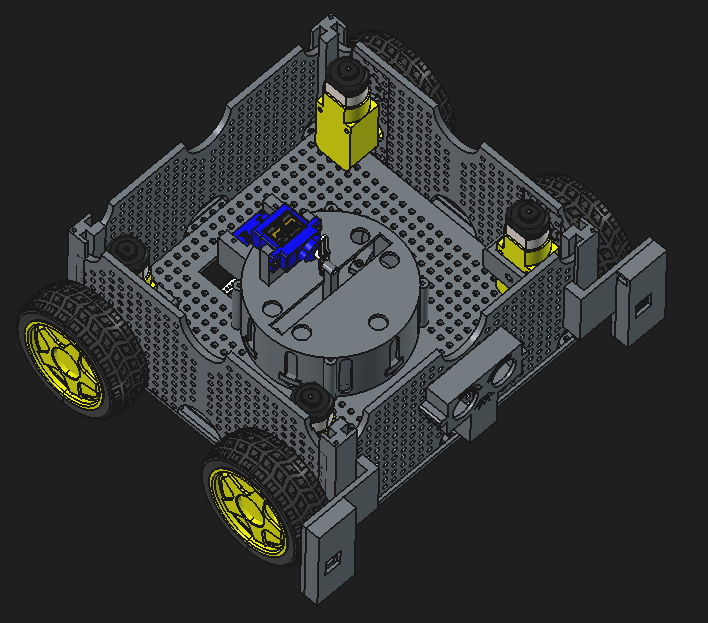
\includegraphics[width=0.75\textwidth,keepaspectratio,alt={Coasterbot Isometrische Ansicht ohne Deckel}]{Coasterbot_Iso_Draufsicht_ohne_Deckel.png}
\caption{Coasterbot Isometrische Ansicht ohne Deckel}
\label{isometrische-ansicht-ohne-deckel}
\end{figure}

Die Darstellung in Abbildung~\ref{isometrische-ansicht-ohne-deckel} zeigt den Innenaufbau des Roboters ohne die obere
Abdeckung. Im Zentrum ist die runde Aufnahme- und Ausgabemechanik für
die Untersetzer zu erkennen. Sie besteht aus einer beweglichen Scheibe
mit mehreren eingelassenen Magneten. Über einen Servomotor und einen
Schubkurbeltrieb. Dieser Schubkurbeltrieb lässt die bewegliche Scheine
auf und ab verfahren. Durch die Magneten können entsprechende
Untersetzer aufgenommen werden. Es wird ausreichend Platz vorgesehen,
dass wenigsten vier Untersetzer in dieser Mechanik vorgehalten werden.

An den vier Ecken des Chassis sind die Antriebsmotoren der Räder zu
sehen. Die Räder selbst sind mit gelben Felgen ausgestattet und an
seitlichen Halterungen befestigt.

\subsubsection{Untere Ansicht}\label{untere-ansicht}

\begin{figure}
\centering
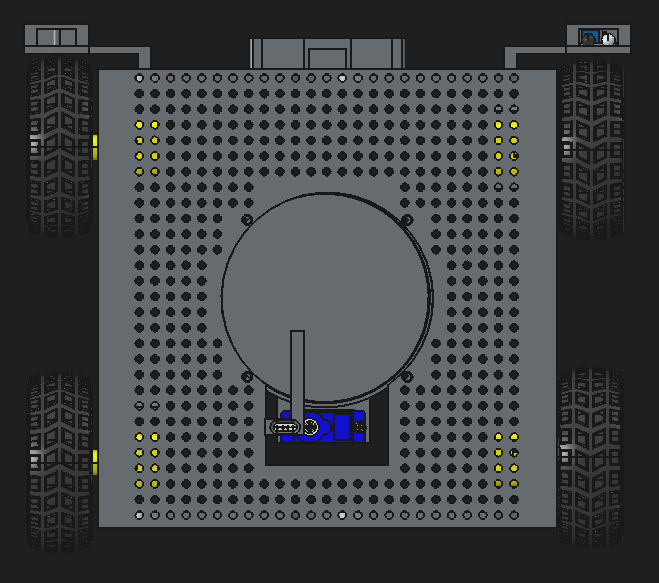
\includegraphics[width=0.75\textwidth,keepaspectratio,alt={Coasterbot untere Ansicht}]{Coasterbot_untere_Ansicht.png}
\caption{Coasterbot untere Ansicht}
\label{untere-ansicht}
\end{figure}

In Abbildung~\ref{untere-ansicht} ist zentral erkennbar die Unterseite der Untersetzer-Mechanik mit dem
herausragenden Auswurf-/Führungssteg sowie dem blauen Servomotor
darunter. Wird ein Untersetzer ausgegeben, wird dieser soweit
heruntergelassen, dass er auf dem Führungssteg abliegt. Damit wird eine
sichere Ausrichtung des Untersetzer gewahrt. Anschließen rotiert der
Servomotor um 90° wodurch die kurze Seite den Untersetzer nach vorne
schiebt. Durch ein anschließendes Anheben des Hebemechanismus, kann der
Untersetze abgelegt werden. Wird ein Untersetzer wieder aufgenommen,
dreht sich der Ausschieber weitere 90° zur Seite, damit der Heber an der
Mechanik vorbeikommt. Dadurch kann der Heber soweit heruntergefahren
werden, bis die Magneten den sich darunter befindlichen Untersetzer
anziehen und damit aufnehmen. Befestigt wird die Mechanik mit dem
Gehäuse über vier Schrauben.

\subsection{Komponentenübersicht}\label{komponentenuxfcbersicht}

{\def\LTcaptype{none} % do not increment counter
\begin{longtable}[]{@{}
  >{\raggedright\arraybackslash}p{(\linewidth - 4\tabcolsep) * \real{0.3333}}
  >{\raggedright\arraybackslash}p{(\linewidth - 4\tabcolsep) * \real{0.3333}}
  >{\raggedright\arraybackslash}p{(\linewidth - 4\tabcolsep) * \real{0.3333}}@{}}
\toprule\noalign{}
\begin{minipage}[b]{\linewidth}\raggedright
Komponente
\end{minipage} & \begin{minipage}[b]{\linewidth}\raggedright
Funktion
\end{minipage} & \begin{minipage}[b]{\linewidth}\raggedright
Position
\end{minipage} \\
\midrule\noalign{}
\endhead
\bottomrule\noalign{}
\endlastfoot
Zentrale Hebe-Mechanik & Aufnahme und Ausgabe der Untersetzer &
Fahrzeugmitte \\
Servomotor zum heben & Antrieb der zentralen Aufnahme-/Ausgabescheibe &
Oberhalb der Drehscheibe \\
4× Radantriebsmotoren & Fortbewegung des Roboters & Je Rad, in den vier
Ecken \\
HC-05-Board & Abstandssensor (Front) & Fahrzeugfront, hinter der
„Gesichts''-Blende \\
LM393-Board (in der Anfrage als „LM939'' bezeichnet) & Kantenerkennung /
Abgrunderkennung & Vor jedem der vier Räder, nicht dargestellt \\
Lochraster-Chassis & Trägerstruktur, flexible Montage aller Komponenten
& Ober- und Unterseite des Fahrzeugs \\
Inertialsensor & Orientierung im Raum & Im Innenraum, nicht
dargestellt \\
Recheneinheit & Auswertung und Steuerung & Im Innenraum, nicht
dargestellt \\
Energieversorgung & Versorgung der Steuerung, Sensorik und Aktorik mit
Energie & Im Innenraum, nicht dargstellt \\
\end{longtable}
}

\subsection{Funktionsprinzip
(geplant)}\label{funktionsprinzip-geplant}

\begin{enumerate}
\def\labelenumi{\arabic{enumi}.}
\tightlist
\item
  Der Roboter bewegt sich mittels der vier Radantriebe autonom im Raum.
\item
  Die Kantenerkennungssensoren (vor jedem Rad) verhindern das
  Herunterfahren von Kanten oder Stufen.
\item
  Der Abstandssensor an der Front erkennt Hindernisse bzw.
  Personen.
\item
  Die zentrale Hebe-Mechanik gibt an der Zielposition einen Untersetzer
  aus bzw. nimmt einen leeren/benutzten Untersetzer wieder auf.
\item
  Über einen Inertialsensor wird der Verfahrweg aufgenommen und zur
  Orientierung verwendet.
\end{enumerate}

\subsection{Offene Punkte}\label{offene-punkte}

\begin{itemize}
\tightlist
\item
  Hinzufügen der fehlenden zwei LM393-Kantenerkennungssensoren.
\item
  Verkabelung und Steuerungslogik (Mikrocontroller, Motortreiber) sind
  noch nicht dargestellt.
\item
  Positionierung der Steurung, Energieversorgung und Inertialsensorik
\end{itemize}

\end{document}
